% This file is generated by the MATLAB m-file laprint.m. It can be included
% into LaTeX documents using the packages graphicx, color and psfrag.
% It is accompanied by a postscript file. A sample LaTeX file is:
%    \documentclass{article}\usepackage{graphicx,color,psfrag}
%    \begin{document}% This file is generated by the MATLAB m-file laprint.m. It can be included
% into LaTeX documents using the packages graphicx, color and psfrag.
% It is accompanied by a postscript file. A sample LaTeX file is:
%    \documentclass{article}\usepackage{graphicx,color,psfrag}
%    \begin{document}% This file is generated by the MATLAB m-file laprint.m. It can be included
% into LaTeX documents using the packages graphicx, color and psfrag.
% It is accompanied by a postscript file. A sample LaTeX file is:
%    \documentclass{article}\usepackage{graphicx,color,psfrag}
%    \begin{document}% This file is generated by the MATLAB m-file laprint.m. It can be included
% into LaTeX documents using the packages graphicx, color and psfrag.
% It is accompanied by a postscript file. A sample LaTeX file is:
%    \documentclass{article}\usepackage{graphicx,color,psfrag}
%    \begin{document}\input{sample_fig}\end{document}
% See http://www.mathworks.de/matlabcentral/fileexchange/loadFile.do?objectId=4638
% for recent versions of laprint.m.
%
% created by:           LaPrint version 3.16 (13.9.2004)
% created on:           24-Nov-2007 12:46:46
% eps bounding box:     15 cm x 11.0193 cm
% comment:              
%
\begin{psfrags}%
\psfragscanon%
%
% text strings:
\psfrag{s02}[b][b]{\color[rgb]{0,0,0}\setlength{\tabcolsep}{0pt}\begin{tabular}{c}Discrete-Time $\Delta\Sigma$M Frequency Response\end{tabular}}%
\psfrag{s03}[t][t]{\color[rgb]{0,0,0}\setlength{\tabcolsep}{0pt}\begin{tabular}{c}Frequency (rad/sample)\end{tabular}}%
\psfrag{s04}[b][b]{\color[rgb]{0,0,0}\setlength{\tabcolsep}{0pt}\begin{tabular}{c}Magnitude (dB)\end{tabular}}%
%
% xticklabels:
\psfrag{x01}[t][t]{0}%
\psfrag{x02}[t][t]{$\pi/4$}%
\psfrag{x03}[t][t]{$\pi/2$}%
%
% yticklabels:
\psfrag{v01}[r][r]{-120}%
\psfrag{v02}[r][r]{-100}%
\psfrag{v03}[r][r]{-80}%
\psfrag{v04}[r][r]{-60}%
\psfrag{v05}[r][r]{-40}%
\psfrag{v06}[r][r]{-20}%
\psfrag{v07}[r][r]{0}%
%
% Figure:
\resizebox{12cm}{!}{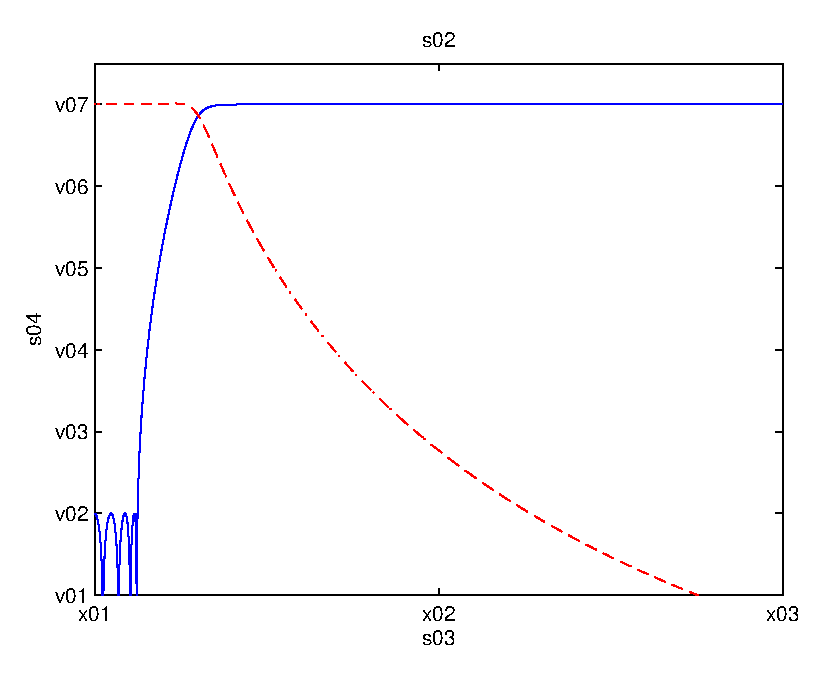
\includegraphics{sample_fig.eps}}%
\end{psfrags}%
%
% End sample_fig.tex
\end{document}
% See http://www.mathworks.de/matlabcentral/fileexchange/loadFile.do?objectId=4638
% for recent versions of laprint.m.
%
% created by:           LaPrint version 3.16 (13.9.2004)
% created on:           24-Nov-2007 12:46:46
% eps bounding box:     15 cm x 11.0193 cm
% comment:              
%
\begin{psfrags}%
\psfragscanon%
%
% text strings:
\psfrag{s02}[b][b]{\color[rgb]{0,0,0}\setlength{\tabcolsep}{0pt}\begin{tabular}{c}Discrete-Time $\Delta\Sigma$M Frequency Response\end{tabular}}%
\psfrag{s03}[t][t]{\color[rgb]{0,0,0}\setlength{\tabcolsep}{0pt}\begin{tabular}{c}Frequency (rad/sample)\end{tabular}}%
\psfrag{s04}[b][b]{\color[rgb]{0,0,0}\setlength{\tabcolsep}{0pt}\begin{tabular}{c}Magnitude (dB)\end{tabular}}%
%
% xticklabels:
\psfrag{x01}[t][t]{0}%
\psfrag{x02}[t][t]{$\pi/4$}%
\psfrag{x03}[t][t]{$\pi/2$}%
%
% yticklabels:
\psfrag{v01}[r][r]{-120}%
\psfrag{v02}[r][r]{-100}%
\psfrag{v03}[r][r]{-80}%
\psfrag{v04}[r][r]{-60}%
\psfrag{v05}[r][r]{-40}%
\psfrag{v06}[r][r]{-20}%
\psfrag{v07}[r][r]{0}%
%
% Figure:
\resizebox{12cm}{!}{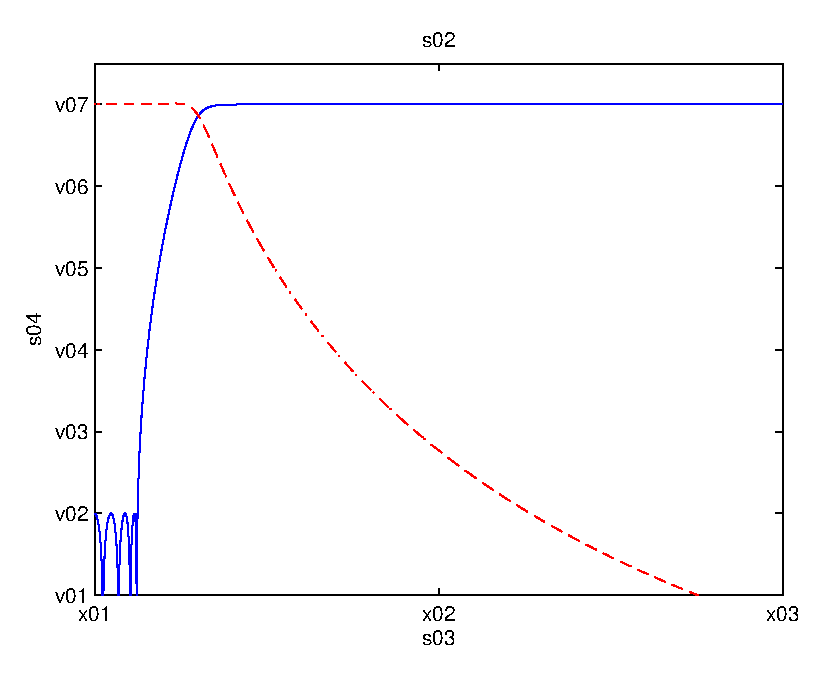
\includegraphics{sample_fig.eps}}%
\end{psfrags}%
%
% End sample_fig.tex
\end{document}
% See http://www.mathworks.de/matlabcentral/fileexchange/loadFile.do?objectId=4638
% for recent versions of laprint.m.
%
% created by:           LaPrint version 3.16 (13.9.2004)
% created on:           24-Nov-2007 12:46:46
% eps bounding box:     15 cm x 11.0193 cm
% comment:              
%
\begin{psfrags}%
\psfragscanon%
%
% text strings:
\psfrag{s02}[b][b]{\color[rgb]{0,0,0}\setlength{\tabcolsep}{0pt}\begin{tabular}{c}Discrete-Time $\Delta\Sigma$M Frequency Response\end{tabular}}%
\psfrag{s03}[t][t]{\color[rgb]{0,0,0}\setlength{\tabcolsep}{0pt}\begin{tabular}{c}Frequency (rad/sample)\end{tabular}}%
\psfrag{s04}[b][b]{\color[rgb]{0,0,0}\setlength{\tabcolsep}{0pt}\begin{tabular}{c}Magnitude (dB)\end{tabular}}%
%
% xticklabels:
\psfrag{x01}[t][t]{0}%
\psfrag{x02}[t][t]{$\pi/4$}%
\psfrag{x03}[t][t]{$\pi/2$}%
%
% yticklabels:
\psfrag{v01}[r][r]{-120}%
\psfrag{v02}[r][r]{-100}%
\psfrag{v03}[r][r]{-80}%
\psfrag{v04}[r][r]{-60}%
\psfrag{v05}[r][r]{-40}%
\psfrag{v06}[r][r]{-20}%
\psfrag{v07}[r][r]{0}%
%
% Figure:
\resizebox{12cm}{!}{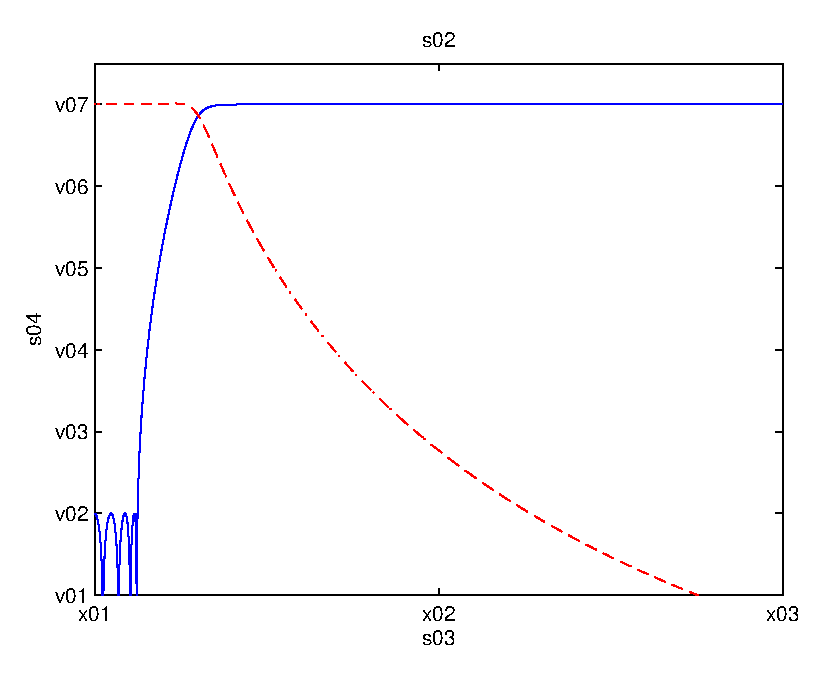
\includegraphics{sample_fig.eps}}%
\end{psfrags}%
%
% End sample_fig.tex
\end{document}
% See http://www.mathworks.de/matlabcentral/fileexchange/loadFile.do?objectId=4638
% for recent versions of laprint.m.
%
% created by:           LaPrint version 3.16 (13.9.2004)
% created on:           24-Nov-2007 12:46:46
% eps bounding box:     15 cm x 11.0193 cm
% comment:              
%
\begin{psfrags}%
\psfragscanon%
%
% text strings:
\psfrag{s02}[b][b]{\color[rgb]{0,0,0}\setlength{\tabcolsep}{0pt}\begin{tabular}{c}Discrete-Time $\Delta\Sigma$M Frequency Response\end{tabular}}%
\psfrag{s03}[t][t]{\color[rgb]{0,0,0}\setlength{\tabcolsep}{0pt}\begin{tabular}{c}Frequency (rad/sample)\end{tabular}}%
\psfrag{s04}[b][b]{\color[rgb]{0,0,0}\setlength{\tabcolsep}{0pt}\begin{tabular}{c}Magnitude (dB)\end{tabular}}%
%
% xticklabels:
\psfrag{x01}[t][t]{0}%
\psfrag{x02}[t][t]{$\pi/4$}%
\psfrag{x03}[t][t]{$\pi/2$}%
%
% yticklabels:
\psfrag{v01}[r][r]{-120}%
\psfrag{v02}[r][r]{-100}%
\psfrag{v03}[r][r]{-80}%
\psfrag{v04}[r][r]{-60}%
\psfrag{v05}[r][r]{-40}%
\psfrag{v06}[r][r]{-20}%
\psfrag{v07}[r][r]{0}%
%
% Figure:
\resizebox{12cm}{!}{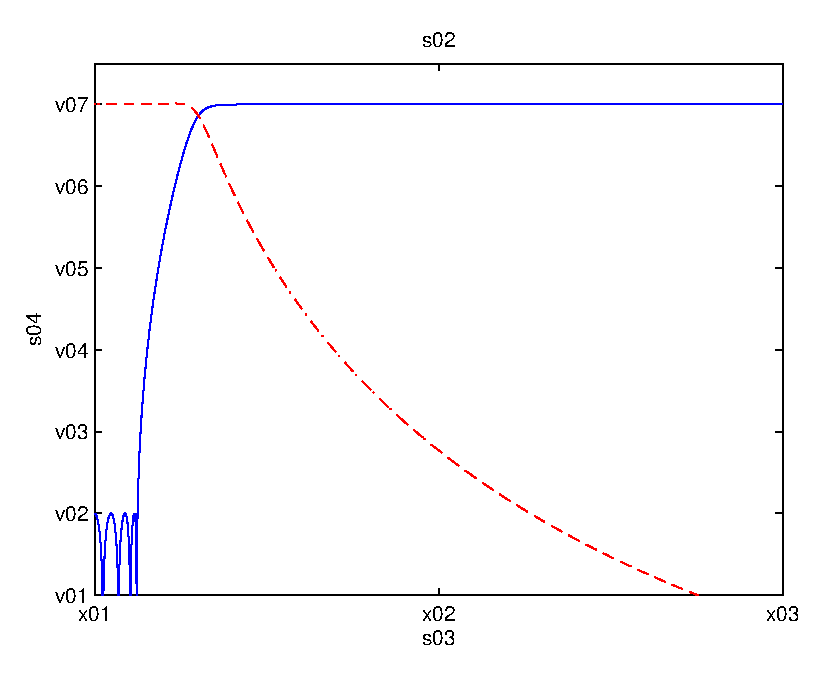
\includegraphics{sample_fig.eps}}%
\end{psfrags}%
%
% End sample_fig.tex
